\chapter{地表输入数据}\label{地表输入数据}
%\addcontentsline{toc}{chapter}{地表输入数据}

%\begin{地表输入数据}
\section{地表覆盖数据}\label{地表覆盖数据}
\subsection{USGS地表覆盖数据}\label{USGS地表覆盖数据}
USGS地表覆盖数据来自美国地质调查局(USGS),数据全称为Global Land Cover Characterization (GLCC) data base Version 2.0 
(https://www.usgs.gov/centers/eros/science\\/usgs-eros-archive-land-cover-products-global-land-cover-characterization-glcc)。
数据为全球 $30''$ (约1公里) 分辨率,经纬度网格,单时次数据,划分类型如表~\ref{tab:USGS覆盖类型} 所示。
% Please add the following required packages to your document preamble:
% \usepackage{booktabs}
\begin{table}[]
\centering
\caption{USGS覆盖类型}
\label{tab:USGS覆盖类型}
\begin{tabular}{@{}lc@{}}
\toprule
编号 & USGS覆盖类型     \\ \midrule
1  & 城市           \\
2  & 干旱农田与牧场      \\
3  & 灌溉农田与牧场      \\
4  & 干旱/灌溉混合农田与牧场 \\
5  & 农田草地过渡带      \\
6  & 农田林地过渡带      \\
7  & 草地           \\
8  & 灌木地          \\
9  & 草地灌木地混合带     \\
10 & 稀疏草原         \\
11 & 落叶阔叶林        \\
12 & 落叶针叶林        \\
13 & 常绿阔叶林        \\
14 & 常绿针叶林        \\
15 & 混合森林         \\
16 & 内陆水体         \\
17 & 草本湿地         \\
18 & 森林湿地         \\
19 & 贫瘠稀疏植被       \\
20 & 草本苔原         \\
21 & 森林苔原         \\
22 & 混合苔原         \\
23 & 裸土苔原         \\
24 & 雪盖或冰川        \\ \bottomrule
\end{tabular}
\end{table}


由于USGS地表覆盖数据为单时次且年代稍远(主要数据源自AVHRR 1992-1993年间),因此辅以其他特定类型地表覆盖数据对USGS地表覆盖进行更新。
包括全球1公里水体和湿地数据(Global Lakes and Wetlands Database: Lakes and Wetlands Grid (Level 3))~\citep{lehner2004development}、
全球1公里冰川数据~\citep{RGIConsortium2017}、全球1公里城市覆盖数据 (MODIS)~\citep{schneider2009new} 和全球1公里高程数据(USGS)。
替换方式是将以上辅助数据中水体、冰川和城市网格直接对USGS地表数据进行替换。USGS高程数据用于判断海洋,即将高程低于0米的地方设置为海洋格点。
如采用USGS地表覆盖类型进行模拟 (LCT方案),其不同类型相关参数请参考附录~\ref{USGS地表覆盖类型相关参数}。

\subsection{IGBP地表覆盖数据}\label{IGBP地表覆盖数据}
IGBP地表覆盖数据来自美国宇航局(NASA)Moderate Resolution Imaging Spectroradiometer 
(MODIS)MCD12Q1 Version 6(The Terra and Aqua combined MODIS Land Cover Type data product)
的数据(https://lpdaac.usgs.gov/products/mcd12q1v006/),该数据(LC\_Type1)是Terra和Aqua两种卫星数据结合产生 
 \citep{Friedl2019}。数据为全球15$''$(约500 m)分辨率,经纬度网格(对原始数据做了投影转换),每年一幅数据,时间范围从2001至今,分类如表 \ref{tab:IGBP覆盖类型} 所示。

\begin{table}[]
\centering
\caption{IGBP覆盖类型}
\label{tab:IGBP覆盖类型}
\begin{tabular}{@{}lc@{}}
\toprule
编号 & IGBP覆盖类型     \\ \midrule
0  & 水体           \\
1  & 常绿针叶林           \\
2  & 常绿阔叶林      \\
3  & 落叶针叶林     \\
4  & 落叶阔叶林 \\
5  & 混合林     \\
6  & 郁闭灌丛      \\
7  & 稀疏灌丛           \\
8  & 稀疏大草原(木本为主)         \\
9  & 稀疏大草原     \\
10 & 草地         \\
11 & 永久性湿地        \\
12 & 耕地        \\
13 & 城市        \\
14 & 耕地和自然植被混合带        \\
15 & 积雪和冰川        \\
16 & 裸土或稀疏植被覆盖       \\ \bottomrule
\end{tabular}
\end{table}


\section{土壤数据}\label{土壤数据}
\subsection{土壤基础数据}\label{土壤基础数据}
土壤基础属性数据采用Global Soil Dataset for Earth System Modeling(GSDE,http://globalchange.bnu.edu.cn/research/soilw) \citep{shangguan2014global}
和SoilGrids (https:\\//www.soilgrids.org/)\citep{poggio2021soilgrids} 两套数据。GSDE采用土壤连接法融合了世界土壤图和多个区域级或国家级的土壤数据库,基于土壤剖面和土壤类型图生成。其空间分辨率为1公里。其垂直层次为8层 (0-0.045, 0.045-0.091, 0.091-0.166, 0.166-0.289, 0.289-0.493, 0.493-0.829, 0.829-1.383, 1.383-2.296 m),这一分层方案与CoLM一致(第一层对应CoLM第一和第二层)。SoilGrids基于土壤剖面和数百个环境协变量图层采用基于机器学习的数字土壤制图方法生成,空间分辨率为250 m。其垂直层次为6层(0-0.05,0.05-0.15,0.15-0.3,0.3-0.6,0.6-1,1-2m)。对两个数据按CoLM的土壤分层方案采用深度加权方法进行了标准化处理。其中第十层无数据,用第九层填补。

\subsection{土壤水热特征参数及尺度转换}\label{土壤水热特征参数及尺度转换}

基于土壤基础数据集GSDE和SoilGrids,CoLM团队开发了全球1 km分辨率土壤水热特征参数数据供陆面模式土壤水热传输过程模拟直接使用。
在土壤热力参数方面,CoLM提供了七种土壤导热率计算方案以供选择,分别为 \citet{farouki1981thermal}方案,\citet{Johansen1975} 方案,
\citet{cote2005} 方案,\citet{balland2005}方案,\citet{lu2007improved} 方案,\citet{tarnawski2012series} 方案和 \citet{de1963thermal} 方案。
根据\citet{dai2019evaluation}的评估结果,\citet{balland2005} 方案的计算结果与土壤导热率观测数据的均方根误差最小,
在CoLM中模拟的土壤温度和地表湍流通量与观测数据最为接近。因此,\citet{balland2005} 方案为CoLM使用的默认方案。
土壤热容量可由固体土壤、液态水和固态水的热容量根据其质量百分比加权得到。
在土壤水力参数方面,CoLM基于两个经典的土壤水分特征曲线模型 \citet{campbell1974} 和 \citet{van1980closed},
选取了针对模型参数的超过30种高被引用或新近开发的土壤转换函数 (PTF, Pedotransfer Function),对模型参数进行最优拟合。
以\citet{balland2005} 和 \citet{campbell1974} 模型为例,两个待定参数通过解下列极值问题得到:
\begin{equation}
\chi\left(\hat{\psi}_{s}, \hat{\lambda}\right)=\min \sum_{i=1}^{N}\left[\psi\left(\hat{\psi}_{s}, \hat{\lambda}\right)-\psi\left(\psi_{s i}, \lambda_{i}\right)\right]^{2}
\end{equation}
%
其中的$\psi_{s i}$, $\lambda_{i}$为每一组PTF的预报结果。通过此方法得到的参数$\hat{\psi}_{s}$, $\hat{\lambda}$是最为接近PTF集合内全部PTF预报结果的参数,
即集合内的最优参数。van Genuchten模型的参数同理可得。饱和土壤导水率的估计仍采用传统的PTF集合中位值法。基于以上方法利用GSDE和SoilGrids陆面基础数据集,
即可生成全球高分辨率(1 km)全球土壤水热特征参数~\citep{dai2019evaluation},直接用于陆面过程模拟。


为使得CoLM可应用于不同分辨率的模拟,针对全球1 km土壤水热参数开发了升尺度算法。在具体实施中,CoLM将针对 \citet{campbell1974} 和 \citet{van1980closed} 建立的
土壤水力特征曲线参数以及 \citet{balland2005} 土壤导热率计算方案中Kersten数-饱和度曲线中的参数实施一种满足参数内部关系自洽的升尺度方法,
即将拟合得到的到达所有细网格曲线距离最短的曲线对应的参数作为表征粗网格特征的最优参数,而饱和土壤导水率/导热率和干土壤导热率采用几何平均法进行聚合。
以升尺度 \citet{campbell1974} 土壤水分特征曲线中的参数为例,具体方法如下:
首先,给出粗网格内所有细网格对应的土壤水分特征曲线,即通过每个细网格中的参数$\psi_{s i}$, $\lambda_{i}$,计算下列土壤水势向量对应的土壤含水量向量:
\begin{equation}
\begin{array}{l}\psi=[-1,-5,-10,-20,-30,-40,-50,-60,-70,-90,-110,-130,-150,-170,\\-210,-300,-345  -690,-1020,-5100,-15300,-20000,-100000,-1000000]\end{array}
\end{equation}
其次,基于以上土壤水势向量对所有细网格的土壤含水量向量做面积加权平均,得到可以表征粗网格土壤水分特征曲线的土壤含水量向量;最后,在粗网格中利用\citet{campbell1974}土壤水分特征曲线关系拟合上述土壤水势向量和平均后的土壤含水量向量,得到粗网格中 \citet{campbell1974} 土壤水分特征曲线关系中的待定参数$\hat{\psi}_{s}$ 和 $\hat{\lambda}$。粗网格的\citet{van1980closed} 土壤水力特征曲线参数可通过上述升尺度方法类似得到。


升尺度土壤导热率计算方案中Kersten数-饱和度曲线参数采用的方法与上述方法略有区别。粗网格的Kersten数由于其计算的非线性性不可直接由细网格的Kersten数平均得到,故升尺度Kersten数-饱和度曲线参数可通过解下列极值问题得到:

\begin{equation}
(\hat{\alpha}, \hat{\beta})=\min \sum_{i=1}^{N}\left[K_{e}(\hat{\alpha}, \hat{\beta})-K_{e}\left(\alpha_{i}, \beta_{i}\right)\right]^{2}
\end{equation}
其中$\alpha_{i}$,  $\beta_{i}$为每一个细网格中Kersten数-饱和度曲线参数,
$\hat{\alpha}$, $\hat{\beta}$为表征粗网格曲线的参数。
通过此方法得到的粗网格参数是最为接近全部细网格计算结果的参数。


以上方法即为升尺度土壤水力特征曲线参数以及Kersten数-饱和度曲线中的参数的方法,
该方法最大优势为升尺度后的参数之间在原有曲线关系中可保持物理关系与细网格的一致性。
\subsection{土壤颜色}\label{土壤颜色}

土壤颜色(反照率)数据来自NCAR CLM5.0模式(mksrf\_soilcolor\-\_histclm52deg025\-\_earthstatmirca\-\_2005.c210808 版),
共20种土壤颜色分类,为全球$30''$ (1公里)分辨率,经纬度网格。每种土壤分类提供可见光、
近红外波段在土壤干旱时和湿润时(土壤水饱和时)的反照率查找表,其数值同NCAR-CLM技术报告表3.3 (2020年3月23日版) \citep{lawrence2018}。


\subsection{基岩深度}\label{基岩深度}

模式的土壤层数可以根据基岩深度数据集进行设定,使得空间上每个格点有不同土壤层数。采用的基岩深度数据为Global Depth to Bedrock Dataset for Earth System Modeling (GDBDESM,http://globalchange.bnu.edu.cn/research/dtb.jsp, \citet{shangguan2017mapping})。该数据集基于土壤剖面、地质钻孔和环境协变量图层采用机器学习的数字土壤制图方法生成,空间分辨率为1公里。


\section{植被结构及属性数据}\label{植被结构及属性数据}
\subsection{叶面积指数数据}\label{叶面积指数数据}
叶面积指数数据来自重处理的MODIS LAI数据~\citep{yuan20143d}。目前模式提供MODIS第5版和第6.1版数据。其中MODIS第5版数据 (MOD15A2) 为全球 $30''$ (1公里) 分辨率,经纬度网格,时间覆盖2000-2016年,时间分辨率为每8天。MODIS第6.1版数据 (MCD15A2H),空间分辨率为全球 $15''$ (约500米),经纬度网格,时间覆盖从2000年至今,时间分辨率每8天或每月。

\subsection{树高数据}\label{树高数据}
树高数据来自2005年Geoscience Laser Altimeter System (GLAS) aboard ICESat 
(Ice, Cloud, and land Elevation Satellite)卫星数据~\citep{simard2011mapping},
全球$30''$ (1公里) 分辨率,经纬度网格,单时次数据。

\subsection{PFT/PC数据及其依赖数据}\label{PFTPC数据及其依赖数据}
模式如采用PFT或PC植被次网格方式运行,则不能像LCT方案一样直接进行地表覆盖类型聚合(图~\ref{fig:次网格聚合方案} LCT方案所示),
需要对每一个细网格地表覆盖类型进行拆解,得到其网格内PFT的组成种类和各自面积占比。
PFT方案则根据细网格计算得到的PFT种类及占比来聚合到模式网格(图~\ref{fig:次网格聚合方案} PFT方案)。
PC聚合方案同LCT,但是PC跟PFT方案一样,对每种LCT内的PFT进行表征 (包括类型和组成比例,图~\ref{fig:次网格聚合方案} PC方案)。
PFT和PC方案采用同样的植被功能型分类,如表~\ref{tab:PFT分类} 所示:
% Please add the following required packages to your document preamble:
% \usepackage{booktabs}
\begin{table}[]
\centering
\caption{植被功能型-PFT分类}
\label{tab:PFT分类}
\begin{tabular}{@{}lc@{}}
\toprule
\multicolumn{1}{c}{编号} & \multicolumn{1}{c}{植被功能型} \\ \midrule
0                      & 裸土                        \\
1                      & 温带常绿针叶林                   \\
2                      & 北方常绿针叶林                   \\
3                      & 北方落叶针叶林                   \\
4                      & 热带常绿阔叶林                   \\
5                      & 温带常绿阔叶林                   \\
6                      & 热带落叶阔叶林                   \\
7                      & 温带落叶阔叶林                   \\
8                      & 北方落叶阔叶林                   \\
9                      & 常绿阔叶灌木                    \\
10                     & 温带落叶阔叶灌木                  \\
11                     & 北方落叶阔叶灌木                  \\
12                     & 极地C3草                     \\
13                     & C3草                       \\
14                     & C4草                       \\
15                     & C3作物                      \\ \bottomrule
\end{tabular}
\end{table}

{
\begin{figure}[]
\centering
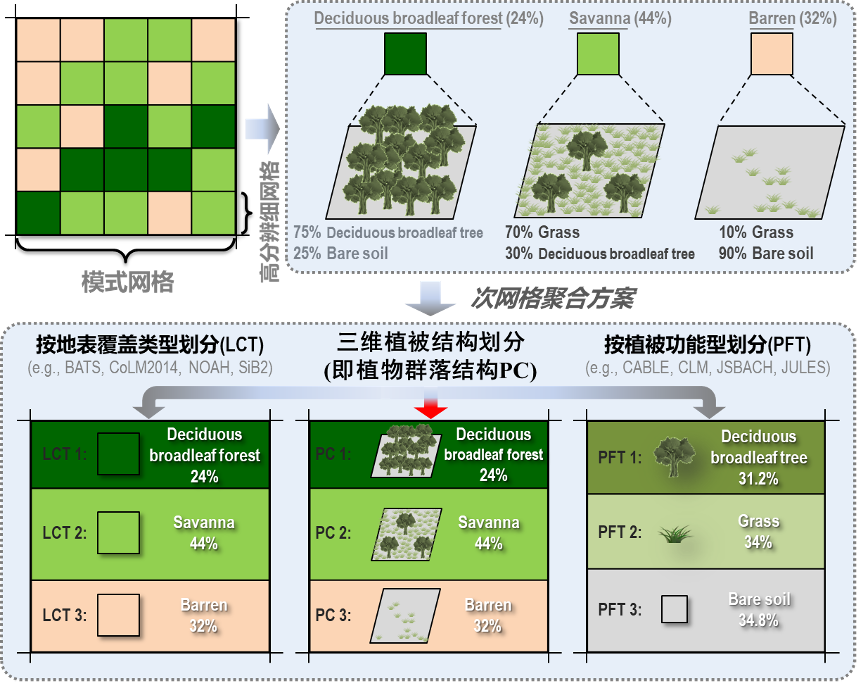
\includegraphics{Figures/地表输入数据/次网格聚合方案.png}
\caption{CoLM三种植被次网格聚合方案 (LCT、PC和PFT) 示意图。}
\label{fig:次网格聚合方案}
\end{figure}
}


由于PFT和PC方案都需要对细网格地表覆盖数据进行PFT分解,而地表覆盖原数据并不包含此信息,
需要借助辅助数据进行计算,其数据来源如表~\ref{tab:网格划分辅助数据}所列。


% Please add the following required packages to your document preamble:
% \usepackage{booktabs}
% \usepackage[table,xcdraw]{xcolor}
% If you use beamer only pass "xcolor=table" option, i.e. \documentclass[xcolor=table]{beamer}
\begin{sidewaystable}[]
\centering
\caption{用于PFT和PC次网格划分辅助数据}
\label{tab:网格划分辅助数据}

\begin{tabular}[h]{p{3cm}p{6cm}p{2cm}p{2cm}p{5cm}}
\toprule
数据名称                                                            & 描述                                                                                              & 分辨率   & 坐标投影               & 参考文献                                            \\ \midrule
MODIS Land Cover Type & The Terra and Aqua combined MODIS Land Cover Type (LC\_Type1) data product, Version 6 (MCD12Q1) & 500 m & Sinusoidal        & (Friedl \& Sulla-Menashe, 2019)                \\\midrule
ESA LC-CCI land cover type                                      & ESA CCI land cover type products                                                                & 300 m & Latitude-Longitude & http://maps.elie.ucl.ac.be \\\midrule
MODIS VCF                                                       & MODIS Vegetation Continuous Fields product, Version 6 (MOD44B)                                           & 250 m & Sinusoidal         & \citet{DiMiceli2015}                        \\\midrule
AVHRR VCF                                                      & AVHRR Tree Cover (evergreen, deciduous and broadleaf, needleleaf) Continuous Fields                      & 1 km  & Latitude-Longitude & \citet{defries2000new}                         \\\midrule
Köppen-Geiger climate classification                                     & Present Köppen-Geiger climate classification maps at 1-km resolution                            & 1 km  & Latitude-Longitude & \citet{beck2018}                            \\\midrule
Reprocessed MODIS LAI                                           & Reprocessed MODIS leaf area index produces, Version 6                                           & 500 m & Sinusoidal         & \citet{yuan2011reprocessing}                              \\\midrule
WorldClim Version2                                             & Worldclim 2: New 1-km spatial resolution climate surfaces for global land areas                          & 1 km  & Latitude-Longitude & \citet{fick2017worldclim}                        \\\midrule
Canopy height                                                   & Global 1 km forest canopy height map                                                            & 1 km  & Latitude-Longitude & \citet{simard2011mapping}                          \\ \bottomrule
\end{tabular}
\end{sidewaystable}
如采用PFT/PC方案进行植被次网格模拟,其不同类型相关参数请参考附录~\ref{植被功能型PFT相关参数} 和附录~\ref{植物群落PC次网格PFT相关参数}。


\section{湖泊深度数据}\label{湖泊深度数据}
湖泊深度数据来自Lake-depth data set Version 2.0~\citep{kourzeneva2012global},数据为全球$30''$ (约1公里)分辨率,经纬度网格,单时次数据。


\section{城市数据}\label{城市数据}

\subsection{城市地表覆盖}\label{城市地表覆盖}
城市地表覆盖数据采用MODIS-IGBP地表覆盖数据(章节 \ref{IGBP地表覆盖数据})中的城市覆盖类型作为判别依据。
模式利用该数据集区分不同年份网格城市覆盖类型,获得城市在网格中的覆盖度,反应不同年份的城市覆盖变化。

\subsection{城市类型划分}\label{城市类型划分}
模式对城市覆盖地区不同城市类型进行细分。城市类型分类数据目前采取两种方案:
\begin{enumerate}
    \item 传统的3类城市——高建筑街区 (Tall Building Distinct, TBD)、高密度(High Density, HD) 和中密度 (Medium Density, MD);
    \item 10类Local Climate Zone (LCZ)分类,如图~\ref{fig:LCZ分类图示}  所示。
\end{enumerate}
{
\begin{figure}[]
\centering
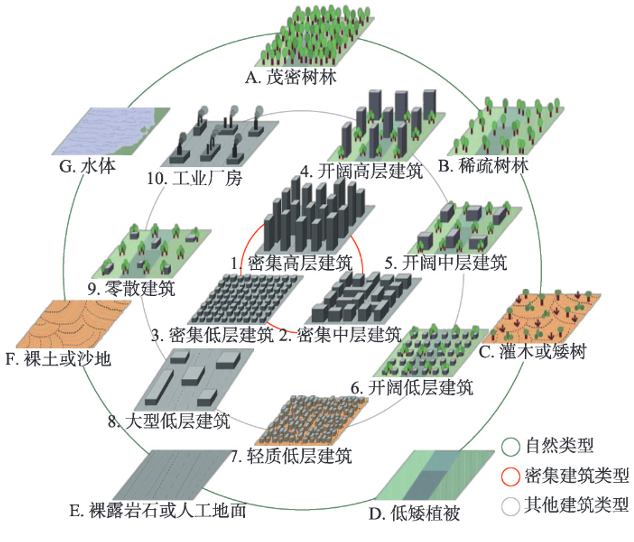
\includegraphics{Figures/地表输入数据/LCZ分类图示.png}
\caption{LCZ分类示意图}
\label{fig:LCZ分类图示}
\end{figure}
}


模式对于传统的城市类型分类与NCAR CLM--Urban Model~\citep{oleson2020parameterization} 相同,
根据 \citet{jackson2013parameterization} 的城市分类数据对全球城市化程度进行分类。该数据集中,城市化有三个水平,
及TBD、HD和MD,每1km格点被划分为三个密度类别之一,通过该数据集对urban patch分为3类。其中,
TBD类城市指至少在1平方公里内,建筑高度全部大于或等于10层楼高且透水面比例较小(5$\sim$15\%);HD类城市建筑高度为3$\sim$10层,
透水面比例通常为5$\sim$25\%,这些地区通常为商业、住宅或工业区;MD类城市建筑高度通常为1$\sim$3层,且透水面比例较高,为20$\sim$60\%。
LCZ数据目前使用的 \citet{demuzere2022global} 全球LCZ分类数据,该数据空间分辨率为100米,
通过向轻量级随机森林模型输入大量标记训练区域和地球观测图像来生成,并对150个选定的功能城市地区采用自助交叉验证和专题基准测试评估了其质量。

\subsection{建筑形态及属性数据}\label{建筑形态及属性数据}
对于城市覆盖而言,建筑物的形态和物理性质(如反照率,导热率等)与其它地表覆盖类型完全不同,
这些物理性质取决于建筑物的材质及城市几何结构数据,比如: 不透水面比例分布(impervious fraction)、
建筑物屋顶面比例分布(roof fraction)、建筑物高度(building height)以及街区宽高比(H/W ratio)、反照率、发射率、导热率以及比热容等等。
目前使用 \citet{oleson2020parameterization} 基于 \citet{jackson2013parameterization} 的建筑数据开发的NCAR城市工具
(Toolbox for Human-Earth SystemIntegration \& Scaling (THESIS) toolset, http://www.cgd.ucar.edu/iam/projects/thesis/thesis-urbanproperties-tool.html)
为模式生成各类城市形态以及物理性质输入参数。
该工具根据一定规则将全球所有国家分为33类 (图~\ref{fig:地区分类}),并根据传统城市分类进一步划分,不同类的国家不同类型建筑具有不同的性质。
%
而LCZ分类本身包含了一些建筑材料信息,不同地区的同类LCZ虽然有差别但是可能不会太大,
因此LCZ形态参数目前采用典型值设定,该部分数据一部分来源于~\citet{stewart2014evaluation},另一部分参考了WRF中的参数设置。
{
\begin{figure}[]
\centering
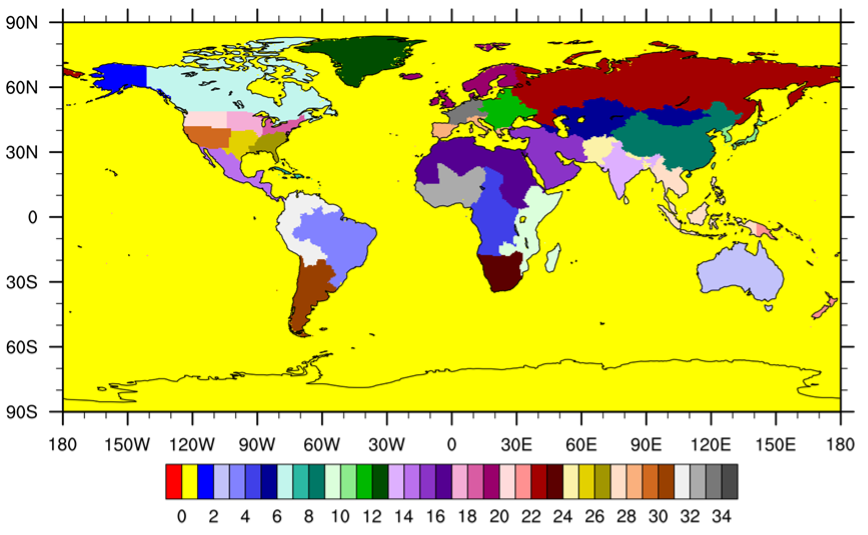
\includegraphics{Figures/地表输入数据/地区分类.png}
\caption{地区分类示意图}
\label{fig:地区分类}
\end{figure}
}


\subsection{城市树覆盖数据}\label{城市树覆盖数据}
NCAR CLM城市数据集比较全面的描述了全球城市的形态特征和物理性质,但是其城市数据缺少关于植被(树)和水体的描述,
LCZ分类虽然有植被描述但通常是一个范围值。由于城市只占全球陆地的1\%左右,相比于自然地表,在大尺度上城市占比仍然比较小,
因此在补充城市内部的植被覆盖数据时,需要尽量选择高分辨率的数据。否则,如果分辨率过低,城市中的植被等信息很可能无法识别。
GFCC Tree Cover (https://lpdaac.usgs.gov/products/gfcc30tcv003/) 提供了
2000年、2005年、2010年和2015年四个年代的全球树木覆盖度信息,分辨率为30m,可用于了解森林变化。
该数据的投影方式为UTM,与陆面模式使用的等经纬度网格不同,需对数据进行投影转换,由UTM投影转换为经纬度投影 ($\sim$0.00025\textdegree)。
经过投影转换后,通过对全球数据每个区域的文件进行读取,并统计500m ($\sim$0.0041667\textdegree)分辨率下30m高分辨网格植被总占比,
对四个年份求平均得到500m分辨率下城市格点的树覆盖数据作为城市模式的基础输入数据。

\subsection{城市内水体数据}\label{城市内水体数据}
基于与城市树覆盖同样的原因,水体数据也需要尽量选择高分辨率数据,30米全球地表覆盖数据GlobeLand30是中国研制的30m空间分辨率全球地表覆盖数据,
2014年发布GlobeLand30 2000和2010版。自然资源部于2017年启动对该数据的更新。目前,GlobeLand30 2020版已发布 (http://www.globallandcover.com/)。
除极地地区外,GlobeLand30同样采用了UTM投影,因此需要进行投影转换,
其中数据覆盖如图~\ref{fig:GlobeLand30数据覆盖示意图} 所示 (除2020年外,其他年份不包含极地地区数据)。
该数据集水体精度最高,达到了92.09\%~\citep{陈军2017},且时空分辨率高,
因此投影转换后用同样的方法生成了水体覆盖度数据作为城市模式的原始数据。
{
\begin{figure}[]
\centering
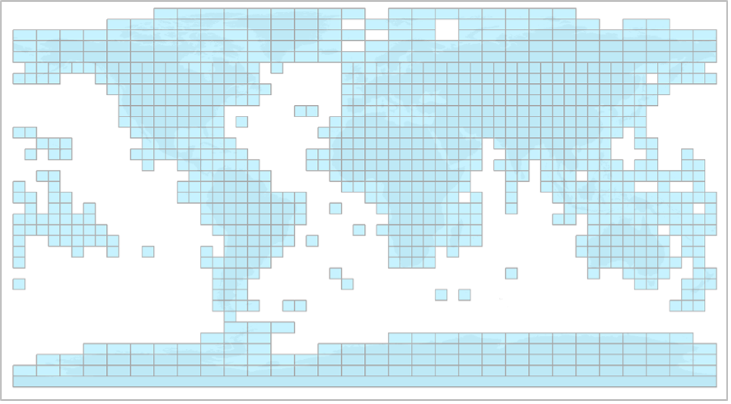
\includegraphics{Figures/地表输入数据/GlobeLand30数据覆盖示意图.png}
\caption{GlobeLand30数据覆盖示意图}
\label{fig:GlobeLand30数据覆盖示意图}
\end{figure}
}

\subsection{城市树高数据}\label{城市树高数据}
树高数据使用的~\citet{simard2011mapping} 全球树高数据,分辨率为1km。除该数据外, \citet{potapov2021mapping} 
利用GEDI卫星数据反演的30m树高数据也同样作为模式树高数据。但由于卫星运行轨道限制,
该数据目前只发布了51.6\textdegree N$\sim$51.6\textdegree S范围内的数据,北半球高纬度地区数据缺失,因此目前该数据集仅作为备用数据。

\subsection{城市LAI/SAI数据}\label{城市LAISAI数据}
由于城市中建筑物的遮掩,卫星反演数据中城市 LAI 存在一定问题,目前模式中城市 LAI 数据利用以下公式根据 0.5\textdegree 范围内的其它PFT (只考虑树,即1-9类PFT)的 LAI/SAI,通过插值并加权平均的办法为城市地区LAI/SAI赋值:
\begin{equation}
L A I_{u r}=\sum_{i=1}^{9} L A I_{P F T_{-} i} \cdot \frac{H T O P_{u r}}{H T O P_{P F T_{-} i}} \cdot P C T_{P F T_{-} i}
\end{equation}
其中$LAI_{PFT_{-}i}$为PFT的LAI(SAI),$HTOP_{ur}$和 $HTOP_{PFT_{-} i}$分别为城市树高和PFT树高,$PCT_{PFT_{-} i}$为PFT占比。城市树木SAI数据采用同样的方法进行计算。


%\end{地表输入数据}
